%%% In this section, you will describe all of the various artifacts that you will generate and maintain during the project life cycle. Describe the purpose of each item below, how the content will be generated, where it will be stored, how often it will be updated, etc. Replace the default text for each section with your own description. Reword this paragraph as appropriate.

\subsection{Major Documentation Deliverables}


\subsubsection{Project Charter}
The Project Charter will have an initial version 1.0 available on 06/28/24. It will be updated monthly to reflect new design developments or changes in system requirements. Each updated version will be released at the end of the month, ensuring that the documentation stays current with the project's progress.

\subsubsection{System Requirements Specification}
The System Requirements Specifications (SRS) will be updated after each prototype is completed, incorporating additional complexity into the project. The aim is to update the SRS every month to account for newly added features and enhancements. This iterative approach ensures that the system requirements evolve in tandem with the project's development, providing a comprehensive and up-to-date guide for the project team. The final version will be delivered with the final designs, the expected date will be 08/20/2024.

\subsubsection{Architectural Design Specification}
The Architectural Design Specification (ADS), which will detail the form factor of the laser harp, has not yet been created. The first version of this document will be available on 07/29/24. It will be created and updated monthly based on the proof-of-concept designs and their iterations. This approach allows for the ADS to adapt and improve with each stage of the project, ensuring that the design specifications align with the evolving prototype. The final version will be available upon the final delivery of the product.

\subsubsection{Detailed Design Specification}
The Detail Design Specification (DDS) will be the circuitry design along with how it fits within its form factor. It will be created and updated monthly based on the proof-of-concept designs and their iterations. This approach allows for the DDS to adapt and improve with each stage of the project, ensuring that the design specifications align with the evolving prototype. The final version will be available upon the final delivery of the product.

\subsection{Recurring Sprint Items}


\subsubsection{Product Backlog}
Items added to the product backlog are based on future needs to complete the project. These items are determined through group decisions and updated by Matthew. The product backlog will be maintained and updated using Google Docs, with notifications sent via Discord. 

\subsubsection{Sprint Planning}
Each sprint will be planned during scheduled breaks. It is estimated that approximately 10 sprints will be needed to complete the project.

\subsubsection{Sprint Goal}
The sprint goal will be determined through group decision, with the customer involved during the sprint planning stages. This ensures that the goals align with both the project objectives and the customer's expectations. 

\subsubsection{Sprint Backlog}
The sprint backlog will be derived from the product backlog, focusing on the next steps needed to complete the project. It will be maintained using Google Workflow to ensure that tasks are organized and progress is tracked efficiently.


\subsubsection{Task Breakdown}
Each individual task will be split based on what can be done without interference from another piece. Team members will voluntarily pick tasks, and any larger task will be handled by two team members to ensure effective collaboration and timely completion.

\subsubsection{Sprint Burn Down Charts}
The burn-down charts will be generated by the SCRUM master assigned to each sprint. The assessment will be based on the accomplishments of each individual team member and will be generated using Excel. These charts will help visualize the progress and remaining work for the sprint, ensuring that the team stays on track to meet its goals. 

\begin{figure}[h!]
    \centering
    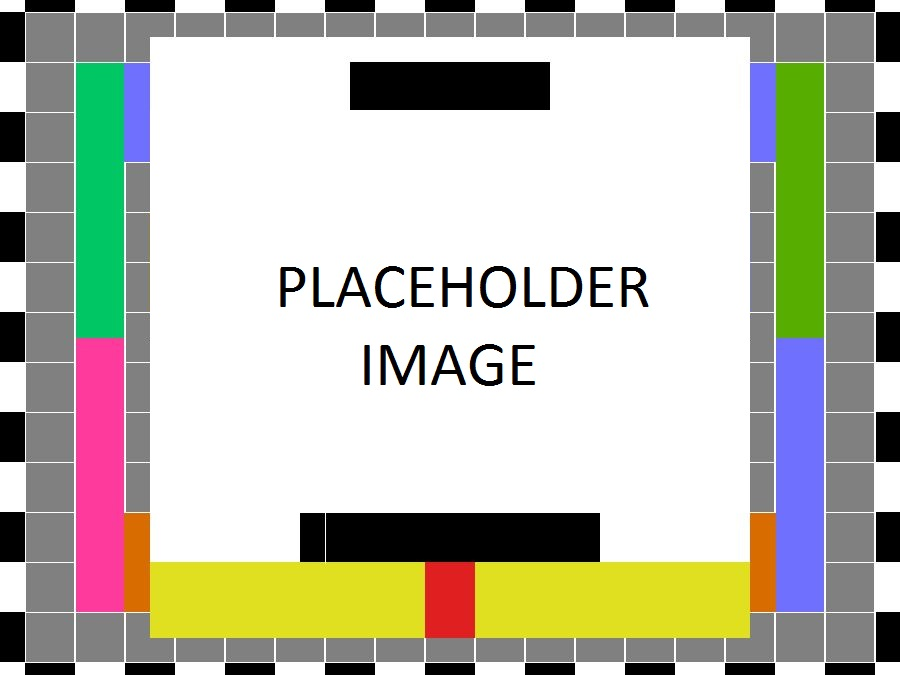
\includegraphics[width=0.5\textwidth]{images/test_image}
    \caption{Example sprint burn down chart}
\end{figure}

\subsubsection{Sprint Retrospective}
The sprint retrospective will involve assessing each burn-down chart to evaluate what tasks were completed. These discussions will occur at the end of each sprint to ensure that all documentation is up to date. The documentation will be compiled into an individual sprint report, summarizing the progress and outcomes of the sprint.

\subsubsection{Individual Status Reports}
Status updates from each individual team member will be provided every three days during each sprint. These updates will include the current task they are working on, the estimated time to completion, and any challenges they are facing. This regular reporting ensures transparency and helps the team address issues promptly.


\subsection{Closeout Materials}


\subsubsection{System Prototype}
The final system prototype will include the finalized Architectural Design Specification (ADS), Detailed Design Specification (DDS), and System Requirements Specifications (SRS). Additionally, the source code will be made available in a GitHub repository. The project will culminate in a demonstration showcasing the use and sound of the laser harp as the final presentation.
\subsubsection{Project Poster}
The project poster will summarize the design parameters, and the purpose of the project, and provide a high-level overview of how the laser harp works. It will serve as a concise visual representation of the project's objectives and achievements.

\subsubsection{Web Page}
The webpage will feature a short demonstration video illustrating the operation of the laser harp. It will also include information on the components required to build this version of the project, providing visitors with a comprehensive overview of the implementation.

\subsubsection{Demo Video}
The demo video will be 5-10 minutes long and will demonstrate how to turn on the laser harp, select different sounds, and play across different octaves. This video will serve as a detailed guide for users interested in understanding the functionality and operation of the laser harp prototype

\subsubsection{Source Code}
The source code will be maintained through GitHub to ensure that all code is updated and accessible to all parties involved. Upon completion of the project, the customer will receive all files, ensuring they have a complete and functional version of the project.
\subsubsection{Source Code Documentation}
Doxygen will be used to generate and keep the coding documentation up to date. This will ensure that the source code is well-documented and easily understandable for future developers and maintainers.

\subsubsection{Hardware Schematics}
Wiring and circuit diagrams will be provided to detail the electrical design of the laser harp. These schematics will be essential for understanding the hardware connections and for troubleshooting or replicating the project.

\subsubsection{CAD Files}
All 3D printed parts and the final form factor will be provided in STL file format. These files will be included in the final project deliverables, allowing for easy reproduction and customization of the physical components.